\documentclass[12pt]{article}
\usepackage[a4paper, top=0.8in, bottom=0.7in, left=0.8in, right=0.8in]{geometry}
\usepackage{amsmath}
\usepackage{amsfonts}
\usepackage{latexsym}
\usepackage{graphicx}
\usepackage{fancyhdr}
\usepackage{tcolorbox}
\usepackage{enumitem}
\usepackage{setspace}
\usepackage[defaultfam,tabular,lining]{montserrat} % Font settings for Montserrat
\usepackage{tikz} % For number line and visual tasks

% General Comment: Template for creating problem sets aligned with a specific standard.

\setlength{\parindent}{0pt}
\pagestyle{fancy}

\setlength{\headheight}{27.11148pt}
\addtolength{\topmargin}{-15.11148pt}

\fancyhf{}
%\fancyhead[L]{\textbf{3.NF.A.1: Understanding Fractions as Numbers}} % Header with standards and topic title
\fancyhead[R]{
\includegraphics[width=0.8cm]{Round Logo.png}} % Placeholder for logo
\fancyfoot[C]{\footnotesize © Study Smart Tutors}

\sloppy

%\newcommand{\dfrac}[2]{\displaystyle\frac{#1}{#2}}

\title{}
\date{}
\hyphenpenalty=10000
\exhyphenpenalty=10000

\begin{document}

\subsection*{Problem Set: Understanding Fractions as Numbers}
\onehalfspacing

% Learning Objective Box
\begin{tcolorbox}[colframe=black!40, colback=gray!5, 
coltitle=black, colbacktitle=black!20, fonttitle=\bfseries\Large, 
title=Learning Objective, halign title=center, left=5pt, right=5pt, top=5pt, bottom=15pt]
\textbf{Objective:} Understand fractions as numbers by interpreting and representing fractions on number lines and visual models.

\end{tcolorbox}
% Exercises Box
\begin{tcolorbox}[colframe=black!60, colback=white, 
coltitle=black, colbacktitle=black!15, fonttitle=\bfseries\Large, 
title=Exercises, halign title=center, left=10pt, right=10pt, top=10pt, bottom=5pt]
\begin{enumerate}[itemsep=1.5em]
    \item Write the fraction that represents \(3\) shaded parts out of \(4\) total parts. 
    \item Mark the fraction \(\displaystyle\frac{1}{2}\) on the number line below.  

    \begin{center}
        \begin{tikzpicture}[x=2cm, y=1cm]
            % Number line
            \draw[thick, ->] (0,0) -- (2,0);
            % Major ticks
            \foreach \x in {0,1,2} {
                \draw[thick] (\x,0.1) -- (\x,-0.1) node[below] {\x};
            }
            % Minor ticks
            \foreach \x in {0.5,1.5} {
                \draw[thick] (\x,0.05) -- (\x,-0.05);
            }
        \end{tikzpicture}
    \end{center}

    \item Write \(\displaystyle\frac{3}{6}\) in simplest form.
    \item Divide the shape below into \(4\) equal parts. \\Shade \(3\) of them to represent \(\displaystyle \frac{3}{4}\).  

    \begin{center}
        \begin{tikzpicture}
            \draw[thick] (0,0) rectangle (4,2); % Draw rectangle
        \end{tikzpicture}
    \end{center}

    \item Write the fraction represented by the point marked on the number line below.

    \begin{center}
        \begin{tikzpicture}[x=2cm, y=1cm]
            % Number line
            \draw[thick, ->] (0,0) -- (2,0);
            % Major ticks
            \foreach \x in {0,1,2} {
                \draw[thick] (\x,0.1) -- (\x,-0.1) node[below] {\x};
            }
            % Minor ticks
            \foreach \x in {.25, 0.5, .75, 1.25, 1.5, 1.75} {
                \draw[thick] (\x,0.05) -- (\x,-0.05);
            }
            % Mark fraction
            \filldraw[red] (1.5,0) circle (3.5pt)  ;
        \end{tikzpicture}
    \end{center}

    \item What fraction is equivalent to \(\displaystyle\frac{2}{4}\)? Write two examples.
    \item Convert \(\displaystyle \frac{5}{10} \) to a decimal.
    \item Write the fraction that represents \(7\) shaded parts out of \(10\) total parts.
\end{enumerate}
 \vspace{2em}
\end{tcolorbox}

\vspace{1cm}

% Problems Box
\begin{tcolorbox}[colframe=black!60, colback=white, 
coltitle=black, colbacktitle=black!15, fonttitle=\bfseries\Large, 
title=Problems, halign title=center, left=10pt, right=10pt, top=10pt, bottom=60pt]
\begin{enumerate}[start=9, itemsep=6em]
    \item Place the following fractions on the number line: \(\displaystyle\frac{1}{3}, \frac{2}{3}, \frac{1}{6}, \frac{5}{6}\).

   \begin{center}
    \begin{tikzpicture}[x=7cm, y=2.5cm] % Adjust x and y scaling here
        % Number line
        \draw[thick, -] (0,0) -- (1,0);
        % Major ticks
        \foreach \x in {0,1} {
            \draw[thick] (\x,0.1) -- (\x,-0.1) node[below] {\x};
        }
        % Minor ticks
        \foreach \x in {0.166,0.333,0.5,0.666,0.833} {
            \draw[thick] (\x,0.05) -- (\x,-0.05);
        }
    \end{tikzpicture}
\end{center}


    \item A pie is cut into \(8\) equal slices. You eat \(3\) slices. Write the fraction of the pie you ate. Is this fraction greater than or less than \(\displaystyle\frac{1}{2}\)? Explain.
    \item Compare the fractions \(\displaystyle\frac{4}{8}\) and \(\dfrac{3}{4}\). Use \(>\), \(<\), or \(=\) to fill in the blank. Explain your reasoning. \vspace{0.5cm}\\ \(\dfrac{4}{8} \quad \_\_\_\quad \frac{3}{4}\).
    
    \item Show \(\dfrac{2}{5}\) and \(\dfrac{4}{10}\) on a number line. Are they equivalent fractions? Explain why.
    \item Convert the fraction \(\dfrac{11}{4}\) into a mixed number. Then plot it on the number line below.

    \begin{center}
        \begin{tikzpicture}[x=1.5cm, y=1cm]
            % Number line
            \draw[thick, ->] (0,0) -- (5,0);
            % Major ticks
            \foreach \x in {0,1,2,3,4,5} {
                \draw[thick] (\x,0.1) -- (\x,-0.1) node[below] {\x};
            }
        \end{tikzpicture}
    \end{center}
\end{enumerate}
\end{tcolorbox}

\vspace{1em}

% Performance Task Box
\begin{tcolorbox}[colframe=black!60, colback=white, 
coltitle=black, colbacktitle=black!15, fonttitle=\bfseries\Large, 
title=Performance Task: Sharing a Cake, halign title=center, left=10pt, right=10pt, top=10pt, bottom=50pt]
You are sharing a cake equally among \(5\) friends. The cake is cut into \(10\) slices.
\begin{enumerate}[itemsep=7em]
    \item Write a fraction that represents how much cake each friend gets.
    \item If you eat \(2\) of your slices, what fraction of the cake do you have left?
    \item Explain how you could use a number line to represent this situation.
    \vspace{3cm}
\end{enumerate}
\end{tcolorbox}

\vspace{1em}

% Reflection Box
\begin{tcolorbox}[colframe=black!60, colback=white, 
coltitle=black, colbacktitle=black!15, fonttitle=\bfseries\Large, 
title=Reflection, halign title=center, left=10pt, right=10pt, top=10pt, bottom=80pt]
How does understanding fractions as numbers help you solve real-world problems? Share one example where fractions can be useful in everyday life.

\vspace{3cm}

\end{tcolorbox}

\end{document}
